% !TeX root = ../main.tex
% -*- coding: utf-8 -*-

\chapter{理论方法}
\label{ch3}

\section{腔磁振子系统的哈密顿量}
本次研究中所考虑的腔磁振子系统是能实现强耦合的微波腔与YIG球耦合的系统,而本节所讨论的哈密顿量来源于Nakamura与Tang课题组的研究\ChangeNotation\cite{PhysRevLett.113.083603Nakamura,PhysRevLett.113.156401Tang,reviewCavityMagnonics}。在实验中使用的毫米尺度YIG球铁磁共振频率在GHz,而金属制微波腔通常会调制到TE101模式来实现腔中微波光场和YIG球的共振耦合。由于腔中光场每次经腔壁反射都会衰减掉一部分的能量,而YIG球也会因为与装置的接触损失一定的磁振子\ChangeNotation,所以需要对腔中光场进行相干驱动以保持系统中的耦合。关于系统耗散的机理我们会在下一节引入,整个的腔磁振子系统示意图如图\ref{FigSetup}所示:磁振子(YIG球)$m$处于腔内驻波$c$的磁场分量最大处,并且腔外还施加了一均匀偏置磁场$B$作用在磁振子上,这两种磁场方向互相垂直,腔外相干驱动源的频率为$\omega_0$,与腔的耦合强度为$\Omega$。
\begin{figure}[htbp]
	\centering
	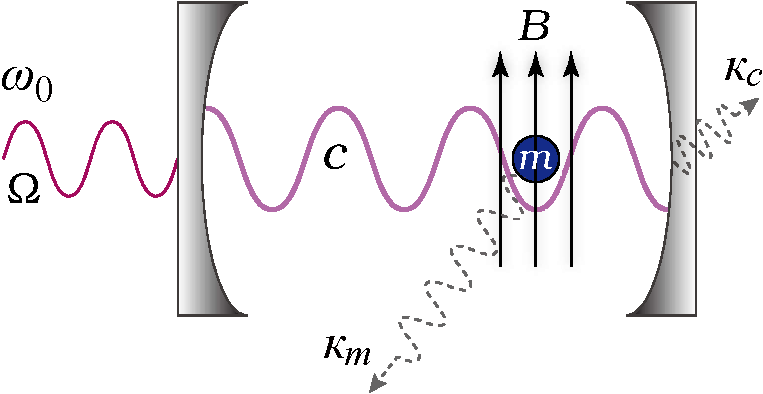
\includegraphics[width=0.5\textwidth,clip]{2_1}
	\caption{腔磁振子系统示意图} 
	\label{FigSetup}
\end{figure}

\subsection{空腔光场的量子化}
我们要想探究系统中的量子特性,就必须对微波腔中的电磁场也就是光场进行二次量子化的处理。在经典场论里介质中的无源电磁场满足Maxwell方程组
\begin{equation}
\begin{aligned}
& \nabla \times \mathbf{H}=\partial \mathbf{D} / \partial t \\
& \nabla \times \mathbf{E}=-\partial \mathbf{B} / \partial t \\
& \nabla \cdot \mathbf{B}=0 \\
& \nabla \cdot \mathbf{D}=0
\end{aligned}\label{Maxwell}
\end{equation}
对于微波腔中的电场分量和磁场分量来说YIG可以看做是各向同性的介质,我们可以得到
\begin{equation}
\mathbf{B} = \mu_{0} \mu \mathbf{H}, \quad \mathbf{D} = \varepsilon_0 \varepsilon \mathbf{E}
\end{equation}
其中$\mu_{0}$,$\varepsilon_0$分别是真空中的磁导率和介电常数,$\mu$,$\varepsilon$分别是YIG的磁导率和相对介电常数。从Maxwell方程组\eqref{Maxwell}中我们可以得到库伦规范$\nabla\cdot\mathbf{A}(\mathbf{r}, t)=0$下的波动方程
\begin{equation}
\nabla^{2} \mathbf{A}=\mu_{0}\mu \varepsilon_0\varepsilon \partial^{2} \mathbf{A} / \partial t^{2} \label{WaveFunction}
\end{equation}
其中$\mathbf{A}(\mathbf{r}, t)$是电磁场的矢势并且满足
\begin{equation}
\mathbf{E}=-\partial \mathbf{A}(\mathbf{r}, t) / \partial t, \quad \mathbf{B}=\nabla \times \mathbf{A}(\mathbf{r}, t)
\label{EBARelations}
\end{equation}

波动方程\eqref{WaveFunction}的解可以表示为平面波叠加的形式$\mathbf{A}(\mathbf{r}, t) = \sum_{k} \big[A_{k} \mathbf{u}_{k}(\mathbf{r}) e^{-i \omega_{k} t}+ A_{k}^* \mathbf{u}_{k}^*(\mathbf{r}) e^{i \omega_{k} t}\big]$,其中$\omega_{k}$表示角频率,$\mathbf{u}_{k}=e^{i \mathbf{k} \cdot  \mathbf{r}}\mathbf{e}_{k}$,$\mathbf{e}_{k}$为偏振矢量(polarization vector),$\mathbf{k}$为波矢\ChangeNotation。二次量子化的操作就是将复振幅$A_{k}$,$A_{k}^*$替换为湮灭产生算符$c_{k}$,$c_{k}^{\dag}$:
\begin{equation}
\hat{\mathbf{A}}(\mathbf{r}, t)\rightarrow\sum_{k} \left[c_{k} \mathbf{u}_{k}(\mathbf{r}) e^{-i \omega_{k} t}+ c_{k}^{\dag} \mathbf{u}_{k}^*(\mathbf{r}) e^{i \omega_{k} t}\right] 
\label{SecondQuantized}
\end{equation}
在这一形式下使用关系\eqref{EBARelations}计算腔中光场的能量$E_c=1/2 \int_{V}\left(\varepsilon \mathbf{E} \cdot \mathbf{E}+1/\mu \mathbf{B} \cdot \mathbf{B}\right) d V$可以得到光场的哈密顿量\ChangeNotation\cite{gerry2005introductory}
\begin{equation}
\hat{H}_{\mathrm{c}} = \hbar \sum_{k} \omega_{k} c_{k}^{\dag} c_{k}
\label{CavityHamiltonian}
\end{equation}
这里$\hbar$表示普朗克常数,在这个过程中我们需要用空间部分满足的亥姆霍兹方程的解来定出\eqref{SecondQuantized}中的系数\ChangeNotation\cite{reviewCavityMagnonics}
\begin{equation}
\left(\nabla^{2}+k^{2}\right) \mathbf{u}_{k}(\mathbf{r})=0
\label{Helmholtz}
\end{equation}
其解的二维矢量$\mathbf{u}_{k}$满足$\int_{V} \mathbf{u}_{k} \cdot \mathbf{u}_{k^{\prime}}^{*} \mathrm{~d}^{3} r=V \delta_{k, k^{\prime}}$,$V$表示腔的内部体积。亥姆霍兹方程\eqref{Helmholtz}还需要满足周期性边界条件,这取决于具体腔的几何外形和材质。最终定出系数的场算符写作
\begin{align}
&\hat{\mathbf{A}}(\mathbf{r}, t)= \sum_{k} \sqrt{\frac{\hbar}{2 V \varepsilon_{0} \varepsilon \omega_{k}}} \left[ c_{k} \mathbf{u}_{k}(\mathbf{r}) e^{-i \omega_{k} t} + c_{k}^{\dag} \mathbf{u}_{k}^{*} (\mathbf{r}) e^{i \omega_{k} t} \right] \\
&\hat{\mathbf{E}}(\mathbf{r}, t)=i \sum_{k} \sqrt{\frac{\hbar \omega_{k}}{2 V \varepsilon_{0} \varepsilon}} \left[ c_{k} \mathbf{u}_{k}(\mathbf{r}) e^{-i \omega_{k} t} - c_{k}^{\dag} \mathbf{u}_{k}^{*} (\mathbf{r}) e^{i \omega_{k} t} \right] \\
&\hat{\mathbf{B}}(\mathbf{r}, t)=i \sum_{k} \sqrt{\frac{\hbar}{2 V \varepsilon_{0} \varepsilon \omega_{k}}} \left[ c_{k} \mathbf{k} \times \mathbf{u}_{k}(\mathbf{r}) e^{-i \omega_{k} t} - c_{k}^{\dag} \mathbf{k}^* \times \mathbf{u}_{k}(\mathbf{r})^* e^{i \omega_{k} t} \right]
\label{BOperator}
\end{align}

\subsection{自旋波的量子化及与光场的耦合}
处于YIG球中的自旋粒子(spins)之间有着强关联相互作用(strong interactions),这使得它们的集体运动表现出自旋波的行为,类似于声波可以量子化为声子那样,自旋波的量子化激子(excitations)被称作磁振子\ChangeNotation。自旋波的激发会引起宏观上磁性材料磁化强度的变化,我们可以从磁化强度满足的演化方程出发,使用与上一小节类似的方法也可以将YIG球中的自旋波(磁化强度)量子化。

对于在外加偏置磁场$\mathbf{H}_0$中磁化的YIG球,用$\mathbf{M}$表示它的磁化强度,此时材料的自由能可以表示为\cite{reviewCavityMagnonics}
\begin{equation}
\begin{aligned}
E=\int_{V} \mathrm{~d}^{3} r \left[\frac{A}{M_{\mathrm{s}}^{2}} \sum_{i=x, y, z}\left|\nabla M_{i}\right|^{2}+U_{\mathrm{an}}[\mathbf{M}]-\mu_{0} \mathbf{M} \cdot \mathbf{H}_{0}-\frac{\mu_{0}}{2} \mathbf{M} \cdot \mathbf{H}_{\mathrm{d}}[\mathbf{M}]\right]
\label{FreeEnergy}
\end{aligned}
\end{equation}
上式中第一项的积分表示磁化体系的交换能。第二项的积分表示各向异性能,对于常见的易轴各向异性会有正比于$M_z^2$的形式。第三项的积分表示与外加磁场间产生的Zeeman能。最后一项的积分表示退磁自能。从单个自旋的角动量定理可以得到磁化强度在无耗散时的演化方程
\begin{equation}
\dot{\mathbf{M}}=-\gamma \mathbf{M} \times \mu_{0} \mathbf{H}_{0}
\label{NoDissLLEquations}
\end{equation}
其中$\gamma=g_{\mathrm{Z}} \mu_{\mathrm{B}} / \hbar$表示旋磁比,$g_{\mathrm{Z}}$表示玻尔磁子,$\mu_{\mathrm{B}}$是电子的朗德因子。由于YIG的矫顽力很小,很容易达到饱和磁化状态,此时方程\eqref{NoDissLLEquations}的解可以理解为磁化强度在外加磁场限定的方向附近做微小震荡,即$\mathbf{M}(\mathbf{r},t)=\mathbf{M}_{\mathrm{s}}(\mathbf{r})+\delta \mathbf{M}(\mathbf{r}, t)$。此时所做的量子化操作如下\cite{reviewCavityMagnonics}
\begin{equation}
\delta \hat{\mathbf{M}}(\mathbf{r}, t) \rightarrow \frac{M_{\mathrm{s}}}{2} \sum_{\eta}\left[\mathbf{w}_{\eta}(\mathbf{r}) {m}_{\eta}+\mathbf{w}_{\eta}^{*}(\mathbf{r}) {m}_{\eta}^{\dagger}\right]
\label{MOperator}
\end{equation}
其中${m}_{\eta}$,${m}_{\eta}^{\dagger}$分别表示磁振子模式$\eta$下的湮灭和产生算符,$\mathbf{w}_{\eta}$是对应的无量纲振幅\ChangeNotation。同样地用这一形式计算\eqref{FreeEnergy},我们关注的是变分量$\delta \hat{\mathbf{M}}$产生的能量\ChangeNotation,积分项中只会包含$\delta \hat{\mathbf{M}}$的一次和二次项,而一次项的积分我们认为是零,剩下的二次项可以整理为磁振子的哈密顿量
\begin{equation}
\hat{H}_{\mathrm{m}}=\hbar \sum_{\eta} \omega_{\eta} {m}_{\eta}^{\dagger} {m}_{\eta}
\end{equation}
其中$\omega_{\eta}$表示模式${\eta}$磁振子的铁磁共振频率,可由方程\eqref{NoDissLLEquations}得到\cite{kittel2005introduction}。磁化强度算符归一化系数的计算依赖于不同的各向异性考量,具体可以查看参考文献\ChangeNotation\cite{reviewCavityMagnonics}。

现在我们可以来考虑把YIG放置到微波腔中,并且外加偏置磁场使其饱和磁化。此时整个系统能量为\cite{reviewCavityMagnonics}
\begin{equation}
\hat{\mathcal{H}}=\int_V \left(\frac{\varepsilon}{2} \hat{\mathbf{E}}^{2}+\frac{1}{2 \mu} \hat{\mathbf{B}}^{2}-\hat{\mathbf{M}} \cdot \hat{\mathbf{B}}+\hat{\mathcal{H}}_{\mathrm{m}}\right) d \mathbf{r}
\end{equation}
可以看出上式中前两项和最后一项分别表示微波腔中光场和磁振子本身的能量密度,第三项表示磁振子与微波的磁场分量相互作用的Zeeman能。我们将场算符\eqref{BOperator}和\eqref{MOperator}代入其中就能得到腔中光与磁振子相互作用的哈密顿量\ChangeNotation\cite{reviewCavityMagnonics}
\begin{equation}
\hat{H}_{\mathrm{cm}}=\hbar \sum_{k \eta}\left(g_{k \eta} \hat{c}_{k} \hat{m}_{\eta}^{\dagger}+g_{k \eta}^{*} \hat{c}_{k}^{\dagger} \hat{m}_{\eta}\right)
\end{equation}
上式中我们已经通过旋转波近似拿掉了粒子数不守衡的项\ChangeNotation,耦合率$g_{k \eta}$为
\begin{equation}
\hbar g_{k \eta}=-\frac{M_{s}}{2} \sqrt{\frac{\hbar}{2 V \varepsilon_{0} \varepsilon \omega_{k}}} \int d \mathbf{r}\left[\nabla \times \mathbf{u}_{k}(\mathbf{r})\right] \cdot \mathbf{w}_{\eta}^{*}(\mathbf{r})
\end{equation}
不失一般性地,我们可以认为耦合率$g_{k \eta}$是实数。至此,我们得到的腔磁振子系统的总哈密顿量为
\begin{equation}
\begin{aligned}
\hat{H}_{tot}=\hat{H}_{\mathrm{c}}+\hat{H}_{\mathrm{m}}+\hat{H}_{\mathrm{cm}}
\end{aligned}
\end{equation}
由于我们考虑的微波腔一直在被外部光源驱动,所以还需要在哈密顿量中加入持续产生相干光子的驱动项
\begin{equation}
\hat{H}_{\mathrm{D}}=\sum_{p} \hbar \Omega_{p}\left({c}_{p} e^{i \omega_{\mathrm{0}} t}+{c}_{p}^{\dagger} e^{-i \omega_{\mathrm{0}} t}\right)
\end{equation}
其中$\Omega_{p}$是与光源功率$P$有关的参数\ChangeNotation,一般来说$|\Omega_{p}|^2 \propto P$。在我们的研究中主要考虑的是磁振子的基模即Kittel模与一个腔模的耦合,所使用的完整哈密顿量如下
\begin{equation}
H = \hbar\omega_{c}c^{\dag}c+\hbar\omega_{m}m^{\dag}m+\hbar gc^{\dag}m+\hbar gm^{\dag}c+i\hbar\Omega(c^{\dag}e^{-i\omega_{0}t}-ce^{i\omega_{0}t})
\label{Hamiltonian}
\end{equation}
其中$\omega_{c}$,$\omega_{m}$分别表示单个腔模和磁振子模的频率,$g$表示它们之间的耦合率。YIG球中Kittel模频率与偏置磁场满足关系$\omega_{m}=\gamma\mu_{0} \mathbf{H}_{0}=\gamma B$。

\section{主方程}
\label{secMaster}
上一节中得到的腔磁振子系统的哈密顿量\eqref{Hamiltonian}只是一个理想化的封闭模型,实际中由于需要对腔中光场进行不断的驱动与测量,系统会不可避免地受到外部环境的影响。通常来说,外部环境会转移或是吸收内部系统的能量,从而导致系统的耗散以及退相干。在量子力学中有多种方法可以用来处理这样的开放量子系统,但是由于我们想了解腔磁振子系统中量子态的具体特点,必须要使用既能描述纯态又能描述混态的密度算符,这样一来合适的方法就是这一节所要论述的主方程。

\subsection{Liouville--von Neumann方程的解}
为了在模型中加入环境的影响,我们可以假设系统$S$和外部环境$R$的耦合具有如下形式的哈密顿量:
\begin{equation}
\mathcal{H}=H_{S}+H_{R}+H_{S R}
\label{Hsr}
\end{equation}
这里$H_{S}$和$H_{R}$分别是系统和环境的哈密顿量,$H_{SR}$为相互作用的哈密顿量。我们可以先不拘泥于环境哈密顿量的具体形式,只需要知道它可以表示为温度和能量的函数。我们的目标是在无需关注环境具体状态的情形下研究混合体系$S \otimes R$中目标系统$S$的演化。为了做到这一点,需要用到密度算符的工具。我们用$\chi(t)$表示$S \otimes R$的密度算符并对环境的部分求迹,定义约化密度算符为
\begin{equation}
\rho(t) \equiv \operatorname{tr}_{R}[\chi(t)]
\end{equation}
显然,如果我们有了约化密度算符$\rho(t)$,很容易就能算出系统$S$的Hilbert空间中任一算符$\hat{O}$的平均,而不需要知道$\chi(t)$的具体形式:
\begin{equation}
\langle\hat{O}\rangle=\operatorname{tr}_{S \otimes R}[\hat{O} \chi(t)]=\operatorname{tr}_{S}\left\{\hat{O} \operatorname{tr}_{R}[\chi(t)]\right\}=\operatorname{tr}_{S}[\hat{O} \rho(t)]
\end{equation}
接下来我们要做的是得到$\rho(t)$的演化方程。

%Schr\"{o}dinger
已知$\chi$的Liouville--von Neumann方程为
\begin{equation}
\dot{\chi}=\frac{1}{i \hbar}[\mathcal{H}, \chi]
\label{LMEq1}
\end{equation}
这里可以把$\mathcal{H}$中的$H_{S}+H_{R}$看作主要部分,$H_{SR}$当成次要部分,转入相互作用绘景下来方便我们的处理:
\begin{equation}
\tilde{\chi}(t) \equiv e^{(i / \hbar)\left(H_{S}+H_{R}\right) t} \chi(t) e^{-(i / \hbar)\left(H_{S}+H_{R}\right) t}
\end{equation}
结合\eqref{Hsr}、\eqref{LMEq1}与上式后可以得到
\begin{align}
\dot{\tilde{\chi}} &=\frac{i}{\hbar}\left(H_{S}+H_{R}\right) \tilde{\chi}-\frac{i}{\hbar} \tilde{\chi}\left(H_{S}+H_{R}\right)+e^{(i / \hbar)\left(H_{S}+H_{R}\right) t} \dot{\chi} e^{-(i / \hbar)\left(H_{S}+H_{R}\right) t} \notag \\
&=\frac{1}{i \hbar}\left[\tilde{H}_{S R}(t), \tilde{\chi}\right]
\label{LMEq2}
\end{align}
% oOSRHH{\ttfamily oOSRHH}{\sffamily oOSRHH}
其中$\tilde{H}_{S R}(t)$是显含时间的量:
\begin{equation}
\tilde{H}_{S R}(t) \equiv e^{(i / \hbar)\left(H_{S}+H_{R}\right) t} H_{S R} e^{-(i / \hbar)\left(H_{S}+H_{R}\right) t}
\end{equation}
对方程\eqref{LMEq2}直接积分可以得到
\begin{equation}
\tilde{\chi}(t)=\chi(0)+\frac{1}{i \hbar} \int_{0}^{t} d t^{\prime}\left[\tilde{H}_{S R}\left(t^{\prime}\right), \tilde{\chi}\left(t^{\prime}\right)\right]
\end{equation}
把上式回代到方程\eqref{LMEq2}的等号右侧:
\begin{equation}
\dot{\tilde{\chi}}=\frac{1}{i \hbar}\left[\tilde{H}_{S R}(t), \chi(0)\right]-\frac{1}{\hbar^{2}} \int_{0}^{t} d t^{\prime}\left[\tilde{H}_{S R}(t),\left[\tilde{H}_{S R}\left(t^{\prime}\right), \tilde{\chi}\left(t^{\prime}\right)\right]\right]
\label{LMExpd2}
\end{equation}
以上的推导都是严格的,我们甚至可以重复\eqref{LMEq2}到\eqref{LMExpd2}的过程来得到无限多的积分项,但是这里做到二阶就足够引入我们下面的近似了。

\subsection{Born--Markov近似}
假设$t=0$时的系统$S$和环境$R$之间没有关联但是相互作用已然存在,我们可以把$\chi(0)=\tilde{\chi}(0)$表示为
\begin{equation}
\chi(0)=\rho(0) R_{0}
\end{equation}
其中$R_{0}$是初始时刻环境的密度矩阵。记$\tilde{\chi}(t)$求迹后的密度矩阵为$\tilde{\rho}(t)$:
\begin{equation}
\operatorname{tr}_{R}[\tilde{\chi}(t)]=e^{(i / \hbar) H_{S} t} \rho(t) e^{-(i / \hbar) H_{S} t} \equiv \tilde{\rho}(t)
\label{InitialAssumption}
\end{equation}
对方程\eqref{LMExpd2}进行求迹运算后我们就可以得到如下的主方程:
\begin{equation}
\dot{\tilde{\rho}}=-\frac{1}{\hbar^{2}} \int_{0}^{t} d t^{\prime} \operatorname{tr}_{R}\left\{\left[\tilde{H}_{S R}(t),\left[\tilde{H}_{S R}\left(t^{\prime}\right), \tilde{\chi}\left(t^{\prime}\right)\right]\right]\right\}
\label{MasterEq}
\end{equation}
这里我们已经通过假设$\operatorname{tr}_{R}\left[\tilde{H}_{S R}(t) R_{0}\right]=0$消去了\eqref{LMExpd2}中的第一项。这项假设需要相互作用$H_{S R}$在$R_{0}$态下的平均值为零,我们总是可以满足这个条件,只用在哈密顿量里考虑是否加入$\operatorname{tr}_{R}\left(H_{S R} R_{0}\right)$即可。

虽然已经假设了初始时$S$和$R$无关,但由于相互作用的存在,之后的时刻里必然会出现新的关联,我们需要在这里引入Born近似。Born近似要求系统和环境间的相互作用是微弱的,这样一来系统就几乎不会对环境有反作用的影响。在这一近似下,环境的状态不随时间改变并且在相互作用中也一直保持不变。此外,Born近似也意味着在处理$\chi(t)$受到的环境影响时只包含$H_{SR}$的同阶量。这样一来,我们就可以把$\tilde{\chi}(t)$写作
\begin{equation}
\tilde{\chi}(t)=\tilde{\rho}(t) R_{0}+O\left(H_{S R}\right)
\end{equation}
这也可以等价的表述为:系统与环境的整体态$\tilde{\chi}(t)$的未来仅由系统态$\tilde{\rho}(t)$决定,而不依赖于环境态的历史。把Born近似应用于方程\eqref{MasterEq}并忽略掉$H_{S R}$的高阶项可以得到
\begin{equation}
\dot{\tilde{\rho}}=-\frac{1}{\hbar^{2}} \int_{0}^{t} d t^{\prime} \operatorname{tr}_{R}\left\{\left[\tilde{H}_{S R}(t),\left[\tilde{H}_{S R}\left(t^{\prime}\right), \tilde{\rho}\left(t^{\prime}\right) R_{0}\right]\right]\right\}
\label{MasterEqBorn}
\end{equation}

仔细观察上面的方程,我们会发现$\tilde{\rho}(t)$依赖于它自身的历史$\tilde{\rho}\left(t^{\prime}\right)$。换句话说,方程\eqref{MasterEqBorn}并不是Markov型的。Markov型的系统要求它的未来只取决于它现在的状态。所以我们另一个要做的主要近似就是把$\tilde{\rho}\left(t^{\prime}\right)$替换为$\tilde{\rho}(t)$,这样我们就得到了Born--Markov近似下的主方程:
\begin{equation}
\dot{\tilde{\rho}}=-\frac{1}{\hbar^{2}} \int_{0}^{t} d t^{\prime} \operatorname{tr}_{R}\left\{\left[\tilde{H}_{S R}(t),\left[\tilde{H}_{S R}\left(t^{\prime}\right), \tilde{\rho}(t) R_{0}\right]\right]\right\}
\end{equation}
Markov近似在物理上是合理的。具体来讲,系统$S$之所以依赖于它的历史是因为通过相互作用$H_{SR}$系统的早期态会映照在改变后的环境态上,而随后的早期态又会被改变后的环境态经过相互作用映照下来。但如果环境是一个一直处于热平衡的庞大系统,也就是热库的话,它就不会保持住来自$S$的改变太长时间。这样一来关键就在于比较热库的关联时间与系统$S$能发生明显变化的时间相比是否远远地小。下面来验证一下上述说法。

我们给定相互作用$H_{SR}$一个具体点的形式
\begin{equation}
H_{S R}=\hbar \sum_{i} s_{i} \Gamma_{i}
\label{HsrSpec}
\end{equation}
这里的$s_{i}$是系统$S$的Hilbert空间里的算符,$\Gamma_{i}$是热库$R$的Hilbert空间里的算符。然后依照上一节所述在相互作用表象下有
\begin{equation}
\begin{aligned}
\tilde{H}_{S R}(t) &=\hbar \sum_{i} e^{(i / \hbar)\left(H_{S}+H_{R}\right) t} s_{i} \Gamma_{i} e^{-(i / \hbar)\left(H_{S}+H_{R}\right) t} \\
&=\hbar \sum_{i}\left(e^{(i / \hbar) H_{S} t} s_{i} e^{-(i / \hbar) H_{S} t}\right)\left(e^{(i / \hbar) H_{R} t} \Gamma_{i} e^{-(i / \hbar) H_{R} t}\right) \\
&=\hbar \sum_{i} \tilde{s}_{i}(t) \tilde{\Gamma}_{i}(t)
\label{HsrSpec2}
\end{aligned}
\end{equation}
此时Born近似的主方程\eqref{MasterEqBorn}就变为了
\begin{align}
\dot{\tilde{\rho}}=&-\sum_{i, j} \int_{0}^{t} d t^{\prime} \operatorname{tr}_{R}\left\{\left[\tilde{s}_{i}(t) \tilde{\Gamma}_{i}(t),\left[\tilde{s}_{j}\left(t^{\prime}\right) \tilde{\Gamma}_{j}\left(t^{\prime}\right), \tilde{\rho}\left(t^{\prime}\right) R_{0}\right]\right]\right\} \notag \\
=&-\sum_{i, j} \int_{0}^{t} d t^{\prime}\left\{\tilde{s}_{i}(t) \tilde{s}_{j}\left(t^{\prime}\right) \tilde{\rho}\left(t^{\prime}\right) \operatorname{tr}_{R}\left[\tilde{\Gamma}_{i}(t) \tilde{\Gamma}_{j}\left(t^{\prime}\right) R_{0}\right]\right. \notag \\
&-\tilde{s}_{i}(t) \tilde{\rho}\left(t^{\prime}\right) \tilde{s}_{j}\left(t^{\prime}\right) \operatorname{tr}_{R}\left[\tilde{\Gamma}_{i}(t) R_{0} \tilde{\Gamma}_{j}\left(t^{\prime}\right)\right]-\tilde{s}_{j}\left(t^{\prime}\right) \tilde{\rho}\left(t^{\prime}\right) \tilde{s}_{i}(t) \notag \\
&\left.\times \operatorname{tr}_{R}\left[\tilde{\Gamma}_{j}\left(t^{\prime}\right) R_{0} \tilde{\Gamma}_{i}(t)\right]+\tilde{\rho}\left(t^{\prime}\right) \tilde{s}_{j}\left(t^{\prime}\right) \tilde{s}_{i}(t) \operatorname{tr}_{R}\left[R_{0} \tilde{\Gamma}_{j}\left(t^{\prime}\right) \tilde{\Gamma}_{i}(t)\right]\right\} \notag \\
=&-\sum_{i, j} \int_{0}^{t} d t^{\prime}\left\{\left[\tilde{s}_{i}(t) \tilde{s}_{j}\left(t^{\prime}\right) \tilde{\rho}\left(t^{\prime}\right)-\tilde{s}_{j}\left(t^{\prime}\right) \tilde{\rho}\left(t^{\prime}\right) \tilde{s}_{i}(t)\right]\left\langle\tilde{\Gamma}_{i}(t) \tilde{\Gamma}_{j}\left(t^{\prime}\right)\right\rangle_{R}\right. \label{MasterEqBorn2} \\
&\left.+\left[\tilde{\rho}\left(t^{\prime}\right) \tilde{s}_{j}\left(t^{\prime}\right) \tilde{s}_{i}(t)-\tilde{s}_{i}(t) \tilde{\rho}\left(t^{\prime}\right) \tilde{s}_{j}\left(t^{\prime}\right)\right]\left\langle\tilde{\Gamma}_{j}\left(t^{\prime}\right) \tilde{\Gamma}_{i}(t)\right\rangle_{R}\right\} \notag 
\end{align}
在上式的推导中我们用到了求迹运算的循环特性---$\operatorname{tr}\left( \hat{A} \hat{B} \hat{C} \right)=\operatorname{tr}\left(\hat{C} \hat{A} \hat{B} \right)= \operatorname{tr} \left( \hat{B} \hat{C} \hat{A} \right)$以及简化符号
\begin{equation}
\begin{aligned}
\left\langle\tilde{\Gamma}_{i}(t) \tilde{\Gamma}_{j}\left(t^{\prime}\right)\right\rangle_{R} &=\operatorname{tr}_{R}\left[R_{0} \tilde{\Gamma}_{i}(t) \tilde{\Gamma}_{j}\left(t^{\prime}\right)\right] \\
\left\langle\tilde{\Gamma}_{j}\left(t^{\prime}\right) \tilde{\Gamma}_{i}(t)\right\rangle_{R} &=\operatorname{tr}_{R}\left[R_{0} \tilde{\Gamma}_{j}\left(t^{\prime}\right) \tilde{\Gamma}_{i}(t)\right]
\end{aligned}
\end{equation}
热库的影响在方程\eqref{MasterEqBorn2}中体现为上式的两个关联函数。我们认为关联函数的变化在时间尺度上远快于$\tilde{\rho}(t)$的变化,理想情况下可以取
\begin{equation}
\left\langle\tilde{\Gamma}_{i}(t) \tilde{\Gamma}_{j}\left(t^{\prime}\right)\right\rangle_{R} \propto \delta\left(t-t^{\prime}\right)
\end{equation}
容易看出这样做的效果就等同于我们把$\tilde{\rho}(t^{\prime})$替换为$\tilde{\rho}(t)$。

\subsection{腔磁振子系统的主方程}
我们回到腔磁振子系统的哈密顿量\eqref{Hamiltonian},把热环境看作包含各种频率的谐振子的集合,并且认为系统内的光场和磁振子各自耦合于独立的热库
\begin{equation}
\begin{aligned}
H_S\equiv{}&\hbar\omega_{c}c^{\dag}c+\hbar\omega_{m}m^{\dag}m+\hbar gc^{\dag}m+\hbar gm^{\dag}c \\
&+i\hbar\Omega(c^{\dag}e^{-i\omega_{0}t}-ce^{i\omega_{0}t}) \\
H_{R}\equiv&\sum_{i}\hbar\omega_{i}a_{i}^{\dag}a_{i}+\sum_{j}\hbar\omega_{j}b_{j}^{\dag}b_{j} \\
H_{SR}\equiv&\sum_{i}g_{c,i}(c^{\dag}a_{i}+a_{i}^{\dag}c)+\sum_{j}g_{m,j}(m^{\dag}b_{j}+b_{j}^{\dag}m)
\label{HamCMRes}
\end{aligned}
\end{equation}
其中$a(a^{\dag})$,$b(b^{\dag})$分别为光子和谐振子热库的湮灭(产生)算符,$\omega_{i}$,$\omega_{j}$表示它们的频率,光子和谐振子与热库的耦合率分别为$g_{c,i}$,$g_{m,j}$。假设热库处于热平衡的温度为$T$,则其密度算符表示为
\begin{equation}
R_{0}=\prod_{i} e^{-\hbar \omega_{i} a_{i}^{\dag}a_{i} / k_{B} T}\left(1-e^{-\hbar \omega_{i} / k_{B} T}\right) \otimes \prod_{j} e^{-\hbar \omega_{j} b_{j}^{\dag}b_{j} / k_{B} T}\left(1-e^{-\hbar \omega_{j} / k_{B} T}\right)
\label{ThermalState}
\end{equation}
其中$k_{B}$表示玻尔兹曼常数,$R_{0}$即为满足玻色--爱因斯坦分布的密度算符。值得注意的是,关于\eqref{HamCMRes}中的$H_{SR}$,这里已经通过旋转波近似略去了粒子数不守衡的项,但是对于有着超强耦合的系统这一近似就不再成立,具体的讨论见相关研究\cite{PhysRevA.98.053834Ridolfo}。

把哈密顿量\eqref{HamCMRes}对照上一小节\eqref{HsrSpec}的形式表示为
\begin{equation}
\begin{gathered}
s_{1}=c, \quad s_{2}=c^{\dagger}, \quad s_{3}=m, \quad s_{4}=m^{\dagger} \\
\Gamma_{1}= \sum_{i} g_{c,i} a_{i}^{\dag}, \quad \Gamma_{2}= \sum_{i} g_{c,i} a_{i}, \quad \Gamma_{3}= \sum_{j} g_{m,j} b_{j}^{\dag}, \quad \Gamma_{4}= \sum_{j} g_{m,j} b_{j}
\end{gathered}
\end{equation}
然后\eqref{HsrSpec2}中的算符就变为了
\begin{equation}
\begin{aligned}
&\tilde{s}_{1}(t)=e^{(i / \hbar) H_{S} t} c e^{-(i / \hbar) H_{S} t} \approx e^{i \omega_{c}c^{\dag}c t} e^{i \omega_{m}m^{\dag}m t} c e^{-i \omega_{c}c^{\dag}c t} e^{-i \omega_{m}m^{\dag}m t} = c e^{-i \omega_{c} t} \\
&\tilde{s}_{2}(t)=e^{(i / \hbar) H_{S} t} c^{\dagger} e^{-(i / \hbar) H_{S} t} \approx e^{i \omega_{c}c^{\dag}c t} e^{i \omega_{m}m^{\dag}m t} c^{\dagger} e^{-i \omega_{c}c^{\dag}c t} e^{-i \omega_{m}m^{\dag}m t} = c^{\dagger} e^{i \omega_{c} t} \\
&\tilde{s}_{3}(t)=e^{(i / \hbar) H_{S} t} m e^{-(i / \hbar) H_{S} t} \approx e^{i \omega_{c}c^{\dag}c t} e^{i \omega_{m}m^{\dag}m t} m e^{-i \omega_{c}c^{\dag}c t} e^{-i \omega_{m}m^{\dag}m t} = m e^{-i \omega_{m} t} \\
&\tilde{s}_{4}(t)=e^{(i / \hbar) H_{S} t} m^{\dagger} e^{-(i / \hbar) H_{S} t} \approx e^{i \omega_{c}c^{\dag}c t} e^{i \omega_{m}m^{\dag}m t} m^{\dagger} e^{-i \omega_{c}c^{\dag}c t} e^{-i \omega_{m}m^{\dag}m t} =m^{\dagger} e^{i \omega_{m} t}
\label{interactS}
\end{aligned}
\end{equation}
以及
\begin{equation}
\begin{aligned}
\tilde{\Gamma}_{1}(t) &=\exp \left(i \sum_{n}\omega_{n}a_{n}^{\dag}a_{n} t\right) \sum_{i} g_{c,i} a_{i}^{\dag} \exp \left(-i \sum_{m}\omega_{m}a_{m}^{\dag}a_{m} t\right) =\sum_{i} g_{c,i} a_{i}^{\dag} e^{i \omega_{i} t} \\
\tilde{\Gamma}_{2}(t) &=\exp \left(i \sum_{n}\omega_{n}a_{n}^{\dag}a_{n} t\right) \sum_{i} g_{c,i} a_{i} \exp \left(-i \sum_{m}\omega_{m}a_{m}^{\dag}a_{m} t\right) =\sum_{i} g_{c,i} a_{i} e^{-i \omega_{i} t} \\
\tilde{\Gamma}_{3}(t) &=\exp \left(i \sum_{n}\omega_{n}b_{n}^{\dag}b_{n} t\right) \sum_{j} g_{m,j} b_{j}^{\dag} \exp \left(-i \sum_{m}\omega_{m}b_{m}^{\dag}b_{m} t\right) =\sum_{j} g_{m,j} b_{j}^{\dag} e^{i \omega_{j} t} \\
\tilde{\Gamma}_{4}(t) &=\exp \left(i \sum_{n}\omega_{n}b_{n}^{\dag}b_{n} t\right) \sum_{j} g_{m,j} b_{j} \exp \left(-i \sum_{m}\omega_{m}b_{m}^{\dag}b_{m} t\right) =\sum_{j} g_{m,j} b_{j} e^{-i \omega_{j} t}
\label{interactGam}
\end{aligned}
\end{equation}
在\eqref{interactS}的推导中我们用到了$H_S$中耦合项与驱动项远远小于光子和谐振子谐振能量的假设,在下一章节的参数选取时我们会知道这在实验上是合理的,而在\eqref{interactGam}的推导中我们则用到了不同模式谐振子算符相互对易的特点。另外还需要注意的是,结合\eqref{ThermalState}与\eqref{interactGam}可以得到$\left\langle\tilde{\Gamma}_{1}(t)\right\rangle_{R_0}=\left\langle\tilde{\Gamma}_{2}(t)\right\rangle_{R_0}=\left\langle\tilde{\Gamma}_{3}(t)\right\rangle_{R_0}=\left\langle\tilde{\Gamma}_{4}(t)\right\rangle_{R_0}=0$,也就是说式\eqref{InitialAssumption}的假设是成立的。

现在让我们来继续推导方程\eqref{MasterEqBorn2},由于求和指标需要遍历$i=1,2,3,4$以及$j=1,2,3,4$,故需要计算64项的积分值,好在其中一半以上的项都是能拿掉的,容易计算出
\begin{align}
	\left\langle\tilde{\Gamma}_{1}(t) \tilde{\Gamma}_{3}\left(t^{\prime}\right)\right\rangle_{R_0} &=\left\langle\tilde{\Gamma}_{1}(t) \tilde{\Gamma}_{4}\left(t^{\prime}\right)\right\rangle_{R_0}=\left\langle\tilde{\Gamma}_{2}(t) \tilde{\Gamma}_{3}\left(t^{\prime}\right)\right\rangle_{R_0}=\left\langle\tilde{\Gamma}_{2}(t) \tilde{\Gamma}_{4}\left(t^{\prime}\right)\right\rangle_{R_0}=0 
	\label{zeroCorrelations} \\
	\left\langle\tilde{\Gamma}_{3}(t) \tilde{\Gamma}_{1}\left(t^{\prime}\right)\right\rangle_{R_0} &=\left\langle\tilde{\Gamma}_{4}(t) \tilde{\Gamma}_{1}\left(t^{\prime}\right)\right\rangle_{R_0}=\left\langle\tilde{\Gamma}_{3}(t) \tilde{\Gamma}_{2}\left(t^{\prime}\right)\right\rangle_{R_0}=\left\langle\tilde{\Gamma}_{4}(t) \tilde{\Gamma}_{2}\left(t^{\prime}\right)\right\rangle_{R_0}=0
\end{align}
以及
\begin{equation}
\left\langle\tilde{\Gamma}_{1}(t) \tilde{\Gamma}_{1}\left(t^{\prime}\right)\right\rangle_{R_0} =\left\langle\tilde{\Gamma}_{2}(t) \tilde{\Gamma}_{2}\left(t^{\prime}\right)\right\rangle_{R_0}=\left\langle\tilde{\Gamma}_{3}(t) \tilde{\Gamma}_{3}\left(t^{\prime}\right)\right\rangle_{R_0}=\left\langle\tilde{\Gamma}_{4}(t) \tilde{\Gamma}_{4}\left(t^{\prime}\right)\right\rangle_{R_0}=0
\label{zeroCorrelations2}
\end{equation}
上面的关联函数\eqref{zeroCorrelations}--\eqref{zeroCorrelations2}以及其厄米共轭的值都是零,这样就大大简化了方程的形式,余下不为零的关联函数为
\begin{align}
\left\langle\tilde{\Gamma}_{1}(t) \tilde{\Gamma}_{2}\left(t^{\prime}\right)\right\rangle_{R_0} &=\sum_{i, k} g_{c,i} g_{c,k} e^{i \omega_{i} t} e^{-i \omega_{k} t^{\prime}} \operatorname{tr}_{R}\left(R_{0} a_{i}^{\dag} a_{k}\right) \notag \\
&=\sum_{i} g_{c,i}^{2} e^{i \omega_{i}\left(t-t^{\prime}\right)} \overline{n}_c\left(\omega_{i}, T\right) \label{Correlations1}
\end{align}
\begin{align}
\left\langle\tilde{\Gamma}_{2}(t) \tilde{\Gamma}_{1}\left(t^{\prime}\right)\right\rangle_{R_0} &=\sum_{i, k} g_{c,i} g_{c,k} e^{-i \omega_{i} t} e^{i \omega_{k} t^{\prime}} \operatorname{tr}_{R}\left(R_{0} a_{i} a_{k}^{\dag}\right) \notag \\
&=\sum_{i} g_{c,i}^{2} e^{-i \omega_{i}\left(t-t^{\prime}\right)} \left[\overline{n}_c \left(\omega_{i}, T\right)+1\right]
\end{align}
\begin{align}
\left\langle\tilde{\Gamma}_{3}(t) \tilde{\Gamma}_{4}\left(t^{\prime}\right)\right\rangle_{R_0} &=\sum_{j, k} g_{m,j} g_{m,k} e^{i \omega_{j} t} e^{-i \omega_{k} t^{\prime}} \operatorname{tr}_{R}\left(R_{0} b_{j}^{\dagger} b_{k}\right) \notag \\
&=\sum_{j} g_{m,j}^{2} e^{i \omega_{j}\left(t-t^{\prime}\right)} \overline{n}_m\left(\omega_{j}, T\right)
\end{align}
\begin{align}
\left\langle\tilde{\Gamma}_{4}(t) \tilde{\Gamma}_{3}\left(t^{\prime}\right)\right\rangle_{R_0} &=\sum_{j, k} g_{m,j} g_{m,k} e^{-i \omega_{j} t} e^{i \omega_{k} t^{\prime}} \operatorname{tr}_{R}\left(R_{0} b_{j} b_{k}^{\dagger}\right) \notag \\
&=\sum_{j} g_{m,j}^{2} e^{-i \omega_{j}\left(t-t^{\prime}\right)}\left[\overline{n}_m\left(\omega_{j}, T\right)+1\right] \label{Correlations4}
\end{align}
其中
\begin{equation}
\begin{aligned}
\overline{n}_c\left(\omega_{i}, T\right) &=\operatorname{tr}_{R}\left(R_{0} a_{i}^{\dagger} a_{i}\right)=\frac{e^{-\hbar \omega_{i} / k_{B} T}}{1-e^{-\hbar \omega_{i} / k_{B} T}}
\\
\overline{n}_m\left(\omega_{j}, T\right) &=\operatorname{tr}_{R}\left(R_{0} b_{j}^{\dagger} b_{j}\right)=\frac{e^{-\hbar \omega_{j} / k_{B} T}}{1-e^{-\hbar \omega_{j} / k_{B} T}}
\end{aligned}
\end{equation}
分别为热平衡下光子和磁振子对应温度$T$与模式$\omega_{i}$,$\omega_{j}$下的平均光子数和磁振子数。

非零关联函数\eqref{Correlations1}--\eqref{Correlations4}中需要对所有模式的热库求和,我们用$G_{a(b)}(\omega)$表示光子(磁振子)所处热库的态密度,$G_{a(b)}(\omega) d\omega$表示$\omega$到$\omega+d\omega$频率间隔内的光子(磁振子)数,这样就可以将求和变为积分。在做了变量替换$\tau = t-t^{\prime}$后,Born近似的主方程可以化简为
\begin{equation}
\begin{aligned}
\dot{\tilde{\rho}}={}&-\int_{0}^{t} d \tau \biggl\{\left[c c^{\dagger} \tilde{\rho}(t-\tau)-c^{\dagger} \tilde{\rho}(t-\tau) c\right] e^{-i \omega_{c} \tau}\left\langle\tilde{\Gamma}_1(t) \tilde{\Gamma}_2(t-\tau)\right\rangle_{R_0}+\text { h.c. }\\
&+\left[c^{\dagger} c \tilde{\rho}(t-\tau)-c \tilde{\rho}(t-\tau) c^{\dagger}\right] e^{i \omega_{c} \tau}\left\langle\tilde{\Gamma}_2(t) \tilde{\Gamma}_1(t-\tau)\right\rangle_{R_0}+\text { h.c. } \\
&+\left[m m^{\dagger} \tilde{\rho}(t-\tau)-m^{\dagger} \tilde{\rho}(t-\tau) m\right] e^{-i \omega_{m} \tau}\left\langle\tilde{\Gamma}_3(t) \tilde{\Gamma}_4(t-\tau)\right\rangle_{R_0}+\text { h.c. }\\
&+\left[m^{\dagger} m \tilde{\rho}(t-\tau)-m \tilde{\rho}(t-\tau) m^{\dagger}\right] e^{i \omega_{m} \tau}\left\langle\tilde{\Gamma}_4(t) \tilde{\Gamma}_3(t-\tau)\right\rangle_{R_0}+\text { h.c. } \biggr\}
\label{MasterEqBorn3}
\end{aligned}
\end{equation}
%书中的方程倒数第二项算符的顺序无误
关联函数也化为了
\begin{align}
\left\langle\tilde{\Gamma}_{1}(t) \tilde{\Gamma}_{2}\left(t^{\prime}\right)\right\rangle_{R_0} &=\int_{0}^{\infty} d \omega e^{i \omega \tau} G_a(\omega) g_{c}^{2}(\omega) \overline{n}_c\left(\omega, T\right) \label{} \\
\left\langle\tilde{\Gamma}_{2}(t) \tilde{\Gamma}_{1}\left(t^{\prime}\right)\right\rangle_{R_0} &=\int_{0}^{\infty} d \omega e^{-i \omega \tau} G_a(\omega) g_{c}^{2}(\omega) \left[\overline{n}_c \left(\omega, T\right)+1\right] \\
\left\langle\tilde{\Gamma}_{3}(t) \tilde{\Gamma}_{4}\left(t^{\prime}\right)\right\rangle_{R_0} &=\int_{0}^{\infty} d \omega e^{i \omega \tau} G_b(\omega) g_{m,j}^{2} \overline{n}_m\left(\omega, T\right) \\
\left\langle\tilde{\Gamma}_{4}(t) \tilde{\Gamma}_{3}\left(t^{\prime}\right)\right\rangle_{R_0} &=\int_{0}^{\infty} d \omega e^{-i \omega \tau} G_b(\omega) g_{m,j}^{2} \left[\overline{n}_m\left(\omega, T\right)+1\right] \label{}
\end{align}
%书中这部分的推导有提到积分中的高频平均掉了低频,是因为各个量的相乘关系导致积分时低频的包络都成了0。旋转波近似中有一个高频被平均掉的说法,是因为高频和低频的相加关系。
方程\eqref{MasterEqBorn3}的积分中存在着三种时间尺度,其中热库的关联函数有着极窄的线型\cite{carmichael1999statistical},其有效关联时间$t_R \sim \hbar/k_B T \approx 10^{-12}s$。而在腔磁振子系统中,系统$\tilde{\rho} (t-\tau)$能发生明显变化的时间取决于耦合率以及关联函数,在实验参数中$t_S \sim 10^{-7}s$。振荡项$e^{-i \omega_{c(m)} \tau}$在微波频域内的时间尺度$t_0 \sim 10^{-10}s$。因此在$t_S$时间尺度内对 $\tau$ 积分时$\tilde{\rho}$可以看作是不变的,换句话说,我们可以直接将$\tilde{\rho} (t-\tau)$替换为$\tilde{\rho} (t)$,也就是使用Markov近似将$\tilde{\rho}$从积分中提出来,剩余的项可以积分为
\begin{equation}
\begin{aligned}
&\int_{0}^{t} d \tau \int_{0}^{\infty} d \omega e^{-i\left(\omega-\omega_{c}\right) \tau} G_a(\omega) g_{c}^{2}(\omega) \\
={}&\pi G_a(\omega_c) g_{c}^{2}(\omega_c)+i P \int_{0}^{\infty} d \omega \frac{G_a(\omega) g_{c}^{2}(\omega)}{\omega_{c}-\omega} \\
&\int_{0}^{t} d \tau \int_{0}^{\infty} d \omega e^{-i\left(\omega-\omega_{c}\right) \tau} G_a(\omega) g_{c}^{2}(\omega) \overline{n}_c(\omega, T) \\
={}&\pi G_a(\omega_c) g_{c}^{2}(\omega_c)\overline{n}_c(\omega_c)+i P \int_{0}^{\infty} d \omega \frac{G_a(\omega) g_{c}^{2}(\omega)}{\omega_{c}-\omega} \overline{n}_c(\omega, T) \\
&\int_{0}^{t} d \tau \int_{0}^{\infty} d \omega e^{-i\left(\omega-\omega_{m}\right) \tau} G_b(\omega) g_{m}^{2}(\omega) \\
={}&\pi G_b(\omega_m) g_{m}^{2}(\omega_m)+i P \int_{0}^{\infty} d \omega \frac{G_b(\omega) g_{m}^{2}(\omega)}{\omega_{m}-\omega} \\
&\int_{0}^{t} d \tau \int_{0}^{\infty} d \omega e^{-i\left(\omega-\omega_{m}\right) \tau} G_b(\omega) g_{m}^{2}(\omega) \overline{n}_m(\omega, T) \\
={}&\pi G_b(\omega_m) g_{m}^{2}(\omega_m)\overline{n}_m(\omega_m)+i P \int_{0}^{\infty} d \omega \frac{G_b(\omega) g_{m}^{2}(\omega)}{\omega_{m}-\omega} \overline{n}_m(\omega, T)
\label{IntergralCorrelations}
\end{aligned}
\end{equation}
上面的积分中我们用到了如下的关系式
\begin{equation}
\lim _{t \rightarrow \infty} \int_{0}^{t} d \tau e^{-i\left(\omega-\omega^{\prime}\right) \tau}=\pi \delta\left(\omega-\omega^{\prime}\right)+i \frac{P}{\omega^{\prime}-\omega}
\end{equation}
其中P表示柯西积分主值。

我们定义如下符号
\begin{align}
\Delta_c \equiv P \int_{0}^{\infty} d \omega \frac{G_a(\omega) g_{c}^{2}(\omega)}{\omega_{c}-\omega},
&\quad \Delta_m \equiv P \int_{0}^{\infty} d \omega \frac{G_b(\omega) g_{m}^{2}(\omega)}{\omega_{m}-\omega} \\
\kappa_c \equiv 2 \pi G_a\left(\omega_{c}\right)g_{c}^{2}(\omega_c),
&\quad \kappa_m \equiv 2 \pi G_b\left(\omega_{m}\right)g_{m}^{2}(\omega_m) \\
\overline{n}_c \equiv \overline{n}_c\left(\omega_{c}, T\right),\label{KcKmDefination}
&\quad \overline{n}_m \equiv \overline{n}_m\left(\omega_{m}, T\right)
\end{align}
结合\eqref{MasterEqBorn3}--\eqref{IntergralCorrelations}后,我们就得到了Born--Markov近似下腔磁振子系统的主方程
\begin{equation}
\begin{aligned}
\dot{\tilde{\rho}}={}&-i \Delta_c\left[c^{\dagger} c, \tilde{\rho}\right]+\kappa_c\left(2 c \tilde{\rho} c^{\dagger}-c^{\dagger} c \tilde{\rho}-\tilde{\rho} c^{\dagger} c\right) \\
&+2 \kappa_c \overline{n}_c\left(c \tilde{\rho} c^{\dagger}+c^{\dagger} \tilde{\rho} c-c^{\dagger} c \tilde{\rho}-\tilde{\rho} c c^{\dagger}\right) \\
&-i \Delta_m\left[m^{\dagger} m, \tilde{\rho}\right]+\kappa_m\left(2 m \tilde{\rho} m^{\dagger}-m^{\dagger} m \tilde{\rho}-\tilde{\rho} m^{\dagger} m\right) \\
&+2 \kappa_m \overline{n}_m\left(m \tilde{\rho} m^{\dagger}+m^{\dagger} \tilde{\rho} m-m^{\dagger} m \tilde{\rho}-\tilde{\rho} m m^{\dagger}\right)
\end{aligned}
\end{equation}
这里的$\tilde{\rho}$还依旧是相互作用绘景下的密度算符,通过公式\eqref{InitialAssumption}可以得到
\begin{equation}
\dot{\rho}=\frac{1}{i \hbar}\left[H_{S}, \rho\right]+e^{-(i / \hbar) H_{S} t} \dot{\tilde{\rho}} e^{(i / \hbar) H_{S} t}
\end{equation}
借助上式将$\tilde{\rho}$变换为$\rho$之后,我们就得到了所需的薛定谔绘景下的主方程
\begin{equation}
\begin{aligned}
\dot{\rho}={}&\frac{1}{i \hbar}\left[H_{S}, \rho\right]-i \Delta_c\left[c^{\dagger} c, \rho\right]-i \Delta_m\left[m^{\dagger} m, \rho\right] \\
&+\kappa_c\left(2 c \rho c^{\dagger}-c^{\dagger} c \rho-\rho c^{\dagger} c\right) \\
&+2 \kappa_c \overline{n}_c\left(c \rho c^{\dagger}+c^{\dagger} \rho c-c^{\dagger} c \rho-\rho c c^{\dagger}\right) \\
&+\kappa_m\left(2 m \rho m^{\dagger}-m^{\dagger} m \rho-\rho m^{\dagger} m\right) \\
&+2 \kappa_m \overline{n}_m\left(m \rho m^{\dagger}+m^{\dagger} \rho m-m^{\dagger} m \rho-\rho m m^{\dagger}\right)
\end{aligned}
\end{equation}
上式中的第二项与第三项的作用相当于给系统中的光子和磁振子的共振频率产生一个平移,实际上实验中不会对平移前后的频率做出区分,为了便于讨论,后面的书写中我们也不区分频移。把$\Delta_c$,$\Delta_m$归到$H_S$里,并且采用Lindblad形式书写主方程为
\begin{equation}
\dot{\rho}=\frac{1}{i\hbar}[H_S,\rho]+\mathcal{L}\{\rho\}
\label{MasterEquation}
\end{equation}
其中$\mathcal{L}$为Liouvillian超算符,定义为$\mathcal{L}\{\rho\}=\sum\limits_{o=c,m}[\kappa_{o}(1 +\overline{n}_{o})(2o\rho o^{\dag}-\{o^{\dag}o,\rho\}) +\kappa_{o} \overline{n}_{o} (2o^{\dag}\rho o-\{oo^{\dag},\rho\})]$。

\section{Fokker-Planck方程}
\label{sec3.2}
主方程\eqref{MasterEquation}是由量子力学算符构成的方程,多数情况下直接求解$\rho$会非常困难,即使是数值求解也需要选择合适的一组基来展开才能得到比较好的结果。我们这一节要做的是借助量子力学的相干态表象把这一关于算符的方程转换为关于经典复数变量的微积分方程。

\subsection{Glauber-Sudarshan $P$表象}
首先来看一下相干态$|\alpha\rangle$和$|\beta\rangle$的定义
\begin{equation}
\begin{aligned}
c|\alpha\rangle=\alpha|\alpha\rangle,& \quad\langle\alpha| c^{\dagger}=(c|\alpha\rangle)^{\dagger}=\alpha^{*}\langle\alpha| \\
m|\beta\rangle=\beta|\beta\rangle,& \quad\langle\beta| m^{\dagger}=(m|\beta\rangle)^{\dagger}=\beta^{*}\langle\beta|
\end{aligned}
\end{equation}
即相干态是湮灭算符的本征态。

由于相干态具有超完备性
\begin{equation}
\frac{1}{\pi} \int d^{2} \alpha|\alpha\rangle\langle\alpha|=1, \quad
\frac{1}{\pi} \int d^{2} \beta|\beta\rangle\langle\beta|=1
\end{equation}
所以我们可以在相干态的基下对密度算符$\rho$进行展开
\begin{equation}
\rho=\int d^{2}\alpha d^{2}\beta P(\alpha,\alpha^{*},\beta,\beta^{*},t)|\alpha,\beta\rangle \langle \alpha,\beta| \label{Pfun} 
\end{equation}
上式定义中的表象即为 Glauber-Sudarshan $P$表象,简称为$P$表象,其中的积分定义在整个复平面上,也就是$d^{2} \alpha d^{2} \beta=d(\operatorname{Re}\{\alpha\}) d(\operatorname{Im}\{\alpha\}) d(\operatorname{Re}\{\beta\}) d(\operatorname{Im}\{\beta\})$。$P$表象中的函数$P(\alpha,\alpha^{*},\beta,\beta^{*},t)$是实数,这一点由密度算符$\rho$的厄米性所保证,同时具有如下性质
\begin{equation}
\begin{aligned}
\int d^{2} \alpha d^{2}\beta P &=\int d^{2} \alpha d^{2}\beta \langle\alpha,\beta \mid \alpha,\beta \rangle P \\
&=\operatorname{tr}\left(\int d^{2} \alpha d^{2}\beta |\alpha,\beta\rangle\langle\alpha,\beta| P\right) \\
&=\operatorname{tr}(\rho) \\
&=1
\end{aligned}
\end{equation}
由此我们说$P$函数具有归一化的概率分布的意义,但需要注意的是某些量子态的$P$函数可以是负的,所以我们称之为准概率分布。用准概率分布$P$可以表示任一算符$O$的期望值为
\begin{equation}
\langle{O}\rangle=\int d^{2}\alpha d^{2}\beta P(\alpha,\alpha^{*},\beta,\beta^{*},t)\langle \alpha,\beta|O|\alpha,\beta\rangle
\end{equation}
使用这一方法可以很方便地计算正则序(normal order)算符的期望值,例如$\langle c^{\dagger}c \rangle = \int d^{2}\alpha d^{2}\beta P(\alpha,\alpha^{*};\beta,\beta^{*};t) \langle \alpha,\beta|c^{\dagger}c|\alpha,\beta\rangle = \int d^{2}\alpha d^{2}\beta P(\alpha,\alpha^{*};\beta,\beta^{*};t)\alpha^{*}\alpha$。为方便后面的推导,我们使用如下记号
\begin{equation}
\overline{\alpha^{*}\alpha} = \int d^{2}\alpha d^{2}\beta P\alpha^{*}\alpha = \langle c^{\dagger}c \rangle
\label{MeanDefination}
\end{equation}

此外,关于$P$表象还值得一提的是,Glauber-Sudarshan $P$表象\eqref{Pfun}只是$P$表象的一种形式,原则上可以使用不同的概率分布函数$P$来定义$P$表象的积分\cite{walls2007quantum}。其他的$P$表象如复数$P$表象(complex $P$ representation),正定$P$表象(positive $P$ representation)等在处理非线性系统时很有帮助,但是对于我们这里的系统 \eqref{Hamiltonian},使用\eqref{Pfun}就足够了。

\subsection{腔磁振子系统的Fokker-Planck方程}
现在我们将系统的哈密顿量\eqref{Hamiltonian}以及$P$表象下的密度算符\eqref{Pfun}代入到主方程\eqref{MasterEquation}中
\begin{equation}
\begin{aligned}
\int d^{2}\alpha d^{2}\beta &\frac{\partial P}{\partial t} |\alpha,\beta\rangle \langle \alpha,\beta| \\
= {} &\int d^{2}\alpha d^{2}\beta P \times 
\{ 
-i\omega_{c} \left(c^{\dag}c|\alpha,\beta\rangle \langle \alpha,\beta| - |\alpha,\beta\rangle \langle \alpha,\beta|c^{\dag}c\right) \\
&-i\omega_{m} \left(m^{\dag}m|\alpha,\beta\rangle \langle \alpha,\beta| - |\alpha,\beta\rangle \langle \alpha,\beta|m^{\dag}m\right) \\
&-g \left(c^{\dag}m|\alpha,\beta\rangle \langle \alpha,\beta| - |\alpha,\beta\rangle \langle \alpha,\beta|c^{\dag}m\right) \\
&-g \left(m^{\dag}c|\alpha,\beta\rangle \langle \alpha,\beta| - |\alpha,\beta\rangle \langle \alpha,\beta|m^{\dag}c\right) \\
&+\Omega (c^{\dag}e^{-i\omega_{0}t}|\alpha,\beta\rangle \langle \alpha,\beta|-ce^{i\omega_{0}t}|\alpha,\beta\rangle \langle \alpha,\beta| \\
&-|\alpha,\beta\rangle \langle \alpha,\beta|c^{\dag}e^{-i\omega_{0}t}+|\alpha,\beta\rangle \langle \alpha,\beta|ce^{i\omega_{0}t}) \\
&-\kappa_{c}(1+\overline{n}_{c})(c^{\dag}c|\alpha,\beta\rangle \langle \alpha,\beta|-2c|\alpha,\beta\rangle \langle \alpha,\beta| c^{\dag}+|\alpha,\beta\rangle \langle \alpha,\beta| c^{\dag}c) \\
&-\kappa_{c}\overline{n}_{c}(|\alpha,\beta\rangle \langle \alpha,\beta| cc^{\dag}-2c^{\dag}|\alpha,\beta\rangle \langle \alpha,\beta| c+cc^{\dag}|\alpha,\beta\rangle \langle \alpha,\beta|) \\
&-\kappa_{m}(1+\overline{n}_{m})(m^{\dag}m|\alpha,\beta\rangle \langle \alpha,\beta|-2m|\alpha,\beta\rangle \langle \alpha,\beta| m^{\dag}+|\alpha,\beta\rangle \langle \alpha,\beta| m^{\dag}m) \\
&-\kappa_{m}\overline{n}_{m}(|\alpha,\beta\rangle \langle \alpha,\beta| mm^{\dag}-2m^{\dag}|\alpha,\beta\rangle \langle \alpha,\beta| m+mm^{\dag}|\alpha,\beta\rangle \langle \alpha,\beta|)
\}
\label{master2fp}
\end{aligned}
\end{equation}
接下来推导的关键是把上式中作用在相干态上的算符替换为复变量微分算子,我们需要借助如下的关系式
\begin{equation}
\begin{aligned}
c|\alpha,\beta\rangle\langle \alpha,\beta|=\alpha|\alpha,\beta\rangle\langle \alpha,\beta|, &\quad |\alpha,\beta\rangle \langle\alpha,\beta| c^{\dag}=|\alpha,\beta\rangle\langle \alpha,\beta|\alpha^{*} \\
m|\alpha,\beta\rangle \langle\alpha,\beta|=\beta|\alpha,\beta\rangle\langle \alpha,\beta|, &\quad
|\alpha,\beta\rangle\langle \alpha,\beta|m^{\dag}=|\alpha,\beta\rangle\langle \alpha,\beta|\beta^{*} \\
c^{\dag}|\alpha,\beta\rangle\langle \alpha,\beta|=(\frac{\partial}{\partial\alpha}+\alpha^{*})|\alpha,\beta\rangle\langle \alpha,\beta|, &\quad
|\alpha,\beta\rangle\langle \alpha,\beta|c=(\frac{\partial}{\partial\alpha^{*}}+\alpha)|\alpha,\beta\rangle\langle \alpha,\beta| \\
m^{\dag}|\alpha,\beta\rangle\langle \alpha,\beta|=(\frac{\partial}{\partial\beta}+\beta^{*})|\alpha,\beta\rangle\langle \alpha,\beta|, &\quad
|\alpha,\beta\rangle\langle \alpha,\beta|m=(\frac{\partial}{\partial\beta^{*}}+\beta)|\alpha,\beta\rangle\langle \alpha,\beta|
\end{aligned}
\end{equation}
由此方程\eqref{master2fp}右侧的各项可以化简为
\begin{equation}
\begin{aligned}
\int d^{2}\alpha & d^{2}\beta Pc^{\dag}c|\alpha,\beta\rangle \langle \alpha,\beta| \\
&= \int d^{2}\alpha d^{2}\beta P(|\alpha|^{2}+\alpha\frac{\partial}{\partial\alpha})|\alpha,\beta\rangle \langle \alpha,\beta| \\
&= \int d^{2}\alpha d^{2}\beta \left(|\alpha|^{2}P|\alpha,\beta\rangle \langle \alpha,\beta|+\alpha P(\frac{\partial}{\partial\alpha}|\alpha,\beta\rangle \langle \alpha,\beta|)\right) \\
&= \int d^{2}\alpha d^{2}\beta \left(|\alpha|^{2}P|\alpha,\beta\rangle \langle \alpha,\beta|+(\frac{\partial}{\partial\alpha}\alpha P|\alpha,\beta\rangle \langle \alpha,\beta|)-(\frac{\partial}{\partial\alpha}\alpha P)|\alpha,\beta\rangle \langle \alpha,\beta|\right) \\
&= \int d^{2}\alpha d^{2}\beta \left(|\alpha|^{2}P|\alpha,\beta\rangle \langle \alpha,\beta|-(\frac{\partial}{\partial\alpha}\alpha P)|\alpha,\beta\rangle \langle \alpha,\beta|\right)
\end{aligned}
\end{equation}
\begin{equation}
\begin{aligned}
\int d^{2}\alpha d^{2}\beta & Pcc^{\dag}|\alpha,\beta\rangle \langle \alpha,\beta| \\
&= \int d^{2}\alpha d^{2}\beta \left(|\alpha|^{2}P|\alpha,\beta\rangle \langle \alpha,\beta|-(\frac{\partial}{\partial\alpha}\alpha P)|\alpha,\beta\rangle \langle \alpha,\beta|+|\alpha,\beta\rangle \langle \alpha,\beta|\right)
\end{aligned}
\end{equation}
\begin{equation}
\begin{aligned}
\int d^{2}\alpha d^{2}\beta & P|\alpha,\beta\rangle \langle \alpha,\beta|c^{\dag}c \\
&= \int d^{2}\alpha d^{2}\beta P(|\alpha|^{2}+\alpha^{*}\frac{\partial}{\partial\alpha^{*}})|\alpha,\beta\rangle \langle \alpha,\beta| \\
&= \int d^{2}\alpha d^{2}\beta \left(|\alpha|^{2}P|\alpha,\beta\rangle \langle \alpha,\beta|-(\frac{\partial}{\partial\alpha^{*}}\alpha^{*} P)|\alpha,\beta\rangle \langle \alpha,\beta|\right)
\end{aligned}
\end{equation}
\begin{equation}
\begin{aligned}
\int d^{2}\alpha d^{2}\beta & P|\alpha,\beta\rangle \langle \alpha,\beta|cc^{\dag} \\
&=\int d^{2}\alpha d^{2}\beta \left(|\alpha|^{2}P|\alpha,\beta\rangle \langle \alpha,\beta|-(\frac{\partial}{\partial\alpha^{*}}\alpha^{*} P)|\alpha,\beta\rangle \langle \alpha,\beta|+|\alpha,\beta\rangle \langle \alpha,\beta|\right)
\end{aligned}
\end{equation}
\begin{equation}
\begin{aligned}
\int d^{2}\alpha d^{2}\beta Pc|\alpha,\beta\rangle \langle \alpha,\beta|c^{\dag} = \int d^{2}\alpha d^{2}\beta |\alpha|^{2}P|\alpha,\beta\rangle \langle \alpha,\beta|
\end{aligned}
\end{equation}
\begin{equation}
\begin{aligned}
\int d^{2}\alpha & d^{2}\beta Pc^{\dag}|\alpha,\beta\rangle \langle \alpha,\beta|c \\
&= \int d^{2}\alpha d^{2}\beta P(|\alpha|^{2}+\alpha\frac{\partial}{\partial\alpha}+\alpha^{*}\frac{\partial}{\partial\alpha^{*}}+\frac{\partial^{2}}{\partial\alpha\partial\alpha^{*}}+1)|\alpha,\beta\rangle \langle \alpha,\beta| \\
&= \int d^{2}\alpha d^{2}\beta \Bigl(|\alpha|^{2}P|\alpha,\beta\rangle \langle \alpha,\beta|-(\frac{\partial}{\partial\alpha}\alpha P)|\alpha,\beta\rangle \langle \alpha,\beta|-(\frac{\partial}{\partial\alpha^{*}}\alpha^{*} P)|\alpha,\beta\rangle \langle \alpha,\beta| \\
&+|\alpha,\beta\rangle \langle \alpha,\beta|+\bigl(\frac{\partial}{\partial\alpha}(P\frac{\partial}{\partial\alpha^{*}}|\alpha,\beta\rangle \langle \alpha,\beta|)\bigr)-(\frac{\partial P}{\partial\alpha}\frac{\partial}{\partial\alpha^{*}}|\alpha,\beta\rangle \langle \alpha,\beta|)\Bigr) \\
&= \int d^{2}\alpha d^{2}\beta \Bigl(|\alpha|^{2}P|\alpha,\beta\rangle \langle \alpha,\beta|-(\frac{\partial}{\partial\alpha}\alpha P)|\alpha,\beta\rangle \langle \alpha,\beta|-(\frac{\partial}{\partial\alpha^{*}}\alpha^{*} P)|\alpha,\beta\rangle \langle \alpha,\beta| \\
&+|\alpha,\beta\rangle \langle \alpha,\beta|+\bigl(\frac{\partial}{\partial\alpha}(\frac{\partial}{\partial\alpha^{*}}P|\alpha,\beta\rangle \langle \alpha,\beta|-\frac{\partial P}{\partial\alpha^{*}}|\alpha,\beta\rangle \langle \alpha,\beta|)\bigr) \\
&-\bigl(\frac{\partial}{\partial\alpha^{*}}\frac{\partial P}{\partial\alpha}|\alpha,\beta\rangle \langle \alpha,\beta|-\frac{\partial^{2}P}{\partial\alpha\partial\alpha^{*}}|\alpha,\beta\rangle \langle \alpha,\beta|\bigr)\Bigr) \\
&= \int d^{2}\alpha d^{2}\beta \Bigl(|\alpha|^{2}P|\alpha,\beta\rangle \langle \alpha,\beta|-(\frac{\partial}{\partial\alpha}\alpha P)|\alpha,\beta\rangle \langle \alpha,\beta|-(\frac{\partial}{\partial\alpha^{*}}\alpha^{*} P)|\alpha,\beta\rangle \langle \alpha,\beta| \\
&+|\alpha,\beta\rangle \langle \alpha,\beta|+\frac{\partial^{2}P}{\partial\alpha\partial\alpha^{*}}|\alpha,\beta\rangle \langle \alpha,\beta|)\Bigr)
\end{aligned}
\end{equation}
在以上积分的推导中我们假设了$P(\alpha,\alpha^{*},\beta,\beta^{*},t)$在无穷远处衰减的充分快,使得我们可以去掉那些边界项的积分。把各项积分带回到\eqref{master2fp}中后,我们就将方程里的相干态从算符的作用下分离了出来,对照方程两端的被积函数我们就得到了腔磁振子系统的Fokker-Planck方程
\begin{equation}
\begin{aligned}
\dot{P} &=\frac{\partial}{\partial \alpha}\left[\left(i \omega_{c} \alpha+i g \beta-\Omega e^{-i \omega_{0} t}+\kappa_{c} \alpha\right) P\right] \\
&+\frac{\partial}{\partial \alpha^{*}}\left[\left(-i \omega_{c} \alpha^{*}-i g \beta^{*}-\Omega e^{i \omega_{0} t}+\kappa_{c} \alpha^{*}\right) P\right]+\frac{\partial^{2}}{\partial \alpha \partial \alpha^{*}}\left(2 \kappa_{c} \bar{n}_{c} P\right) \\
&+\frac{\partial}{\partial \beta}\left[\left(i \omega_{m} \beta+i g \alpha+\kappa_{m} \beta\right) P\right] \\
&+\frac{\partial}{\partial \beta^{*}}\left[\left(-i \omega_{m} \beta^{*}-i g \alpha^{*}+\kappa_{m} \beta^{*}\right) P\right]+\frac{\partial^{2}}{\partial \beta \partial \beta^{*}}\left(2 \kappa_{m} \bar{n}_{m} P\right)
\label{Fokker-Planck}
\end{aligned}
\end{equation}
上面的方程和前面得到的主方程\eqref{MasterEquation}是完全等价的,但是在非线性系统中可能会有些差别,具体参见相关研究\cite{PhysRevA.66.033812Drummond}。另外,可以看出Fokker-Planck方程\eqref{Fokker-Planck}是关于$P$函数的含时二阶偏微分方程,我们可以通过假设长时间演化后的稳态形式去掉时间变量来得到系统的稳态解,但是还有另外一种数值方法来得到方程的含时解,那就是随机微分方程。

\section{随机微分方程}
随机微分方程是应用数学领域中非常重要的一类方程,在金融学、电路滤波问题、优化问题等方面都有着广泛的应用。随机微分方程在数学上有着一套严格的定义和证明,详细可参考相关书籍\cite{bernt2012}\cite{gardiner1985handbook},我们这里着重理解概念以及在物理系统中的使用。

\subsection{随机过程与It\^o积分}
我们先考虑一组随机变量序列$X_{1}, X_{2}, \ldots, X_{n}, \ldots$,假如它们对应于一组时刻序列$t_{1}<t_{2}<\cdots<t_{n}<\cdots$,我们就称这一族时间依赖的随机变量$\{X_{t}\}$为一个随机过程。物理学中有一个经典的随机过程,就是布朗运动。我们知道由于随机涨落力的影响,悬浮于液体中的花粉会表现出无规则的运动,即使花粉保持同样的初始条件每次的运动轨迹也不会完全重合。但是当大量花粉从相同的初始状态运动时,每一时刻的花粉位置就表现出统计上的分布规律,也就是一个随机过程。

有了随机过程的概念,我们可以很容易想到随机过程可以有着自己的演化规律,而用来描述这一规律的方程就是随机微分方程。下面来看一个典型的带随机项的方程
\begin{equation}
\dot{X_t}=A(t,X_t)+B(t,X_t)\xi_t
\label{StochasticEq}
\end{equation}
其中的$A$和$B$都是随机变量$X$的解析函数,$\xi_t$是随机的噪声项,每个时刻的值都是随机数且满足一定的随机分布。出于实际上的考虑,比如要求$\xi_t$各个时刻相互独立且一定时间内的联合分布与时间无关等等,数学上并不能直接把$\xi_t$看作是一个“合理”的随机过程。通常把$\xi_t$定义为
\begin{equation}
\xi_t \cdot dt=d W_t
\end{equation}
这里的$W_t$是一个随机过程,也被称为Wiener过程,在$\Delta t$的时间间隔内$\Delta W_t$是一个服从均值为0,方差为 $\Delta t$ 的高斯分布的随机变量\cite{carmichael1999statistical}。借助Wiener过程就可以把方程\eqref{StochasticEq}写为一般的随机微分方程的形式
\begin{equation}
d X_t=A(t,X_t) dt + B(t,X_t) d W_t
\label{StochasticDiff}
\end{equation}
有了微分方程,自然也有相应的积分
\begin{equation}
X_t=X_0 + \int_{0}^{t} A(s,X_s) ds + \int_{0}^{t} B(s,X_s) d W_s
\end{equation}
但是这里的积分是随机变量的积分,尤其是上式中的第二个积分项有着与确定变量积分不同的定义与规则。

考虑如下形式的随机变量积分
\begin{equation}
\int_{t_{0}}^{t} F_{t^{\prime}} d W_{t^{\prime}}
\label{StochasticInt}
\end{equation}
其中$F_{t}$表示一个任意的随机过程。类似于经典积分定义为黎曼和的极限那样,可以用同样的方式定义随机变量的积分。我们把积分限$[t_0,t]$做$i$等份的均匀分割,每个子间隔的长度为$\Delta t=\left(t-t_{0}\right) / i$,并将端点的时刻表示为$t_{k} \equiv t_{0}+k \Delta t,~ k=0, \ldots, i$。子间隔内的时刻可以表示为
\begin{equation}
\tau_{k} \equiv t_{k}+\alpha \Delta t
\end{equation}
其中$\alpha$是0到1之间的数。定义\eqref{StochasticInt}的随机积分为
\begin{equation}
\int_{t_{0}}^{t} F_{t^{\prime}} d W_{t^{\prime}} \equiv \lim\limits_{\Delta t \to 0} \sum_{k=0}^{i-1} F_{\tau_{k}}\left(W_{t_{k+1}}-W_{t_{k}}\right)
\end{equation}
在经典的积分中黎曼和的极限与$\alpha$的选取无关,但是在上述积分中不行,数学上可以证明Wiener过程几乎必然地处处不可微,随机积分的值依赖于$\alpha$。一个好的选择是取$\tau_{k}$为子间隔的左端点,也就是把$\alpha$设置为0,这样选取的积分被称为It\^o积分,即
\begin{equation}
\int_{t_{0}}^{t} F_{t^{\prime}} d W_{t^{\prime}} \equiv \lim\limits_{\Delta t \to 0} \sum_{k=0}^{i-1} F_{t_{k}}\left(W_{t_{k+1}}-W_{t_{k}}\right)
\label{ItoIntegral}
\end{equation}

\subsection{随机微分方程的数值模拟算法}
正如前文所述,随机微分方程描述了一个随机过程,也就是每个时刻的随机变量。而随机变量是满足着一定的统计分布的,对于连续型随机变量需要用概率密度函数来刻画它的特征。那么很自然的,随机微分方程的背后必然有一个等价的关于概率密度函数的方程,数学上称之为Kolmogorov前向方程,在物理里面其实就是Fokker-Planck方程。作为例子,随机微分方程\eqref{StochasticDiff}与Fokker-Planck方程的对应为
\begin{equation}
\frac{\partial P\left(t,X \mid 0,X_{0}\right)}{\partial t} = \left(-\frac{\partial}{\partial X} A+\frac{1}{2} \frac{\partial^{2}}{\partial X^2} BB\right) P\left(t,X \mid 0,X_{0}\right)
\end{equation}
上式中的$P\left(t,X \mid 0,X_{0}\right)$表示条件概率密度函数,微分算子全都是满足确定变量微分规则的经典微分。反过来我们也可以写出Fokker-Planck方程\eqref{Fokker-Planck}所对应的It\^o随机微分方程组
\begin{align}
d{{\alpha}}&=(-i\omega_{c}{\alpha}-ig{\beta}+\Omega e^{-i\omega_{0}t}-\kappa_{c}{\alpha})dt+\sqrt{\kappa_c\overline{n}_{c}}(dW_1+idW_2) \label{sdes1} \\
d{{\alpha^{*}}}&=(i\omega_{c}{\alpha^{*}}+ig{\beta^{*}}+\Omega e^{i\omega_{0}t}-\kappa_{c}{\alpha^{*}})dt+\sqrt{\kappa_c\overline{n}_{c}}(dW_1-idW_2) \\
d{{\beta}}&=(-i\omega_{m}{\beta}-ig{\alpha}-\kappa_{m}{\beta})dt+\sqrt{\kappa_m\overline{n}_{m}}(dW_3+idW_4) \\
d{{\beta^{*}}}&=(i\omega_{m}{\beta^{*}}+ig{\alpha^{*}}-\kappa_{m}{\beta^{*}})dt+\sqrt{\kappa_m\overline{n}_{m}}(dW_3-idW_4) \label{sdes4}
\end{align}
其中$W_i~(i=1,2,3,4)$是互相独立的Wiener过程。

随机微分方程不像通常的微分方程那样拥有确定的时间演化,我们可以通过数值模拟的方法得到每次演化的轨迹,尽管每次的轨迹都不尽相同,但是当模拟的轨迹足够多的时候,轨迹的平均以及高阶矩却会趋向于平滑,这也正是我们想要的平均粒子数和高阶关联的信息。在用算法模拟随机微分方程之前,我们可以先把方程组\eqref{sdes1}--\eqref{sdes4}变换到旋转坐标系下,也就是把随机变量写作$\alpha=\tilde{\alpha}(t) e^{-i\omega_{0}t}, \beta=\tilde{\beta}(t) e^{-i\omega_{0}t}$,这有利于我们去掉系统中高速震荡的影响从而加速后面的模拟,变换后的随机微分方程组写作
\begin{align}
d{\tilde{\alpha}}&=\big(-i(\omega_{c}-\omega_{0})\tilde{\alpha}-ig\tilde{\beta}+\Omega -\kappa_{c}\tilde{\alpha}\big)dt+\sqrt{\kappa_c\overline{n}_{c}}(d\tilde{W}_1+id\tilde{W}_2) \label{RotateSDEs1} \\
d{\tilde{\alpha}^{*}}&=\big(i(\omega_{c}-\omega_{0})\tilde{\alpha}^{*}+ig\tilde{\beta}^{*}+\Omega -\kappa_{c}\tilde{\alpha}^{*}\big)dt+\sqrt{\kappa_c\overline{n}_{c}}(d\tilde{W}_1-id\tilde{W}_2) \\
d{\tilde{\beta}}&=\big(-i(\omega_{m}-\omega_{0})\tilde{\beta}-ig\tilde{\alpha}-\kappa_{m}\tilde{\beta}\big)dt+\sqrt{\kappa_m\overline{n}_{m}}(d\tilde{W}_3+id\tilde{W}_4) \\
d{\tilde{\beta}^{*}}&=\big(i(\omega_{m}-\omega_{0})\tilde{\beta}^{*}+ig\tilde{\alpha}^{*}-\kappa_{m}\tilde{\beta}^{*}\big)dt+\sqrt{\kappa_m\overline{n}_{m}}(d\tilde{W}_3-id\tilde{W}_4) \label{RotateSDEs4}
\end{align}
其中$\tilde{W}_i~(i=1,2,3,4)$也是互相独立的Wiener过程。我们用积分形式表示方程组
\begin{equation}
\begin{aligned}
\int d{\tilde{\alpha}}&=\int \big(-i(\omega_{c}-\omega_{0})\tilde{\alpha}-ig\tilde{\beta}+\Omega -\kappa_{c}\tilde{\alpha}\big)dt^{\prime}+\sqrt{\kappa_c\overline{n}_{c}}(\int d\tilde{W}_1+i\int d\tilde{W}_2) \\
\int d{\tilde{\alpha}^{*}}&=\int \big(i(\omega_{c}-\omega_{0})\tilde{\alpha}^{*}+ig\tilde{\beta}^{*}+\Omega -\kappa_{c}\tilde{\alpha}^{*}\big)dt^{\prime}+\sqrt{\kappa_c\overline{n}_{c}}(\int d\tilde{W}_1-i\int d\tilde{W}_2) \\
\int d{\tilde{\beta}}&=\int \big(-i(\omega_{m}-\omega_{0})\tilde{\beta}-ig\tilde{\alpha}-\kappa_{m}\tilde{\beta}\big)dt^{\prime}+\sqrt{\kappa_m\overline{n}_{m}}(\int d\tilde{W}_3+i\int d\tilde{W}_4) \\
\int d{\tilde{\beta}^{*}}&=\int \big(i(\omega_{m}-\omega_{0})\tilde{\beta}^{*}+ig\tilde{\alpha}^{*}-\kappa_{m}\tilde{\beta}^{*}\big)dt^{\prime}+\sqrt{\kappa_m\overline{n}_{m}}(\int d\tilde{W}_3-i\int d\tilde{W}_4)
\end{aligned}
\end{equation}
这里拿$\int d\tilde{W}_1$简单说明旋转坐标变换后的方程组\eqref{RotateSDEs1}--\eqref{RotateSDEs4}和\eqref{sdes1}--\eqref{sdes4}是等价的,借用It\^o积分的定义\eqref{ItoIntegral}可得
\begin{equation}
\begin{aligned}
\int d\tilde{W}_{1t^{\prime}}=\int e^{i\omega_{0}t^{\prime}} d W_{1t^{\prime}} ={}& \int \left[\cos({\omega_{0}t^{\prime}})+i\sin({\omega_{0}t^{\prime}})\right] d W_{1t^{\prime}} \\
={}& \lim\limits_{\Delta t \to 0} \sum_{k=0}^{i-1} \cos({\omega_{0}t_k})\left(W_{1t_{k+1}}-W_{1t_{k}}\right) \\
&+ \lim\limits_{\Delta t \to 0} \sum_{k=0}^{i-1} i\sin({\omega_{0}t_k})\left(W_{1t_{k+1}}-W_{1t_{k}}\right)
\end{aligned}
\end{equation}
不难看出$\int d\tilde{W}_1$可以写作一系列新的Wiener过程的线性组合,由于高斯分布的和也是高斯分布,所以$\tilde{W}_1$依然是一个Wiener过程\ChangeNotation。独立性可以从协方差看出来:
\begin{equation}
\begin{aligned}
E\bigg(\int d \tilde{W}_{1t^{\prime}} &\int d \tilde{W}_{2t^{\prime}}\bigg) \\
={}&E\left(\int \Re\left\{e^{i\omega_{0}t^{\prime}} (d{W}_{1t^{\prime}}+id{W}_{2t^{\prime}})\right\} \int \Im\left\{e^{i\omega_{0}t^{\prime}}(d{W}_{1t^{\prime}}+id{W}_{2t^{\prime}})\right\}\right) \\
={}& i\int \cos({\omega_{0}t^{\prime}})\sin({\omega_{0}t^{\prime}}) d{t^{\prime}} - i\int \sin({\omega_{0}t^{\prime}})\cos({\omega_{0}t^{\prime}}) d{t^{\prime}} \\
={}&0
\end{aligned}
\end{equation}
上面的推导中需要用到It\^o规则$dW \cdot dW=dt$。

随机微分方程的数值算法和通常的微分方程有着同样的思路,可以用差分来代替微分,当差分的步长足够小时,数值结果就会接近于真实的值。对于随机微分方程\eqref{StochasticDiff},假设初始值已经确定,我们取时间步长为$\Delta t$,并用$\bar{X}_n$表示$n\Delta t$时的计算值,那么最简单的Euler算法可以写为
\begin{equation}
\bar{X}_{n+1}=\bar{X}_n + A \Delta t + B \Delta W_n
\end{equation}
正如前文所述,$\Delta W_n$是一个服从高斯分布的随机数,并且不同时刻的$\Delta W_n$也是独立的。同样的,随机微分方程组\eqref{RotateSDEs1}--\eqref{RotateSDEs4}的Euler算法为
\begin{equation}
\begin{aligned}
\bar{\tilde{\alpha}}_{n+1}&=\bar{\tilde{\alpha}}_{n}+(-i(\omega_{c}-\omega_{0})\bar{\tilde{\alpha}}_{n}-ig\bar{\tilde{\beta}}_{n}+\Omega -\kappa_{c}\bar{\tilde{\alpha}}_{n})\Delta t+\sqrt{\kappa_c\overline{n}_{c}}(\Delta{W}_{1n}+i\Delta{W}_{2n}) \\
\bar{\tilde{\beta}}_{n+1}&=\bar{\tilde{\beta}}_{n}+(-i(\omega_{m}-\omega_{0})\bar{\tilde{\beta}}_{n}-ig\bar{\tilde{\alpha}}_{n}-\kappa_{m}\bar{\tilde{\beta}}_{n})\Delta t+\sqrt{\kappa_m\overline{n}_{m}}(\Delta{W}_{3n}+i\Delta{W}_{4n})
\end{aligned}
\end{equation}
另外两个共轭方程已包含在内。Euler算法虽然简单易理解,但却收敛性较差,在测试中对于我们所选取的参数$1$~ns的计算需要$0.1$~fs的步长才能收敛,对于目标的$400$~ns总时长来说计算机时过于巨大,因此我们需要更高效的算法。随机微分方程的模拟算法方向有很多研究\cite{TOCINO2002219,Kloeden1992numerical},其中一种可接受的算法是高阶Taylor算法,就像通常微分方程的Taylor算法一样,借助Taylor展开将高阶导数引入差分之中就可以得到高阶Taylor算法。只不过由于随机微分方程特殊的微积分规则,它的高阶Taylor展开的形式和通常微分方程是不一样的,但是推导Taylor展开的思路却是一致的,这里不作展开,直接给出方程组\eqref{RotateSDEs1}--\eqref{RotateSDEs4}的二阶弱收敛Taylor算法为
\begin{equation}
\begin{aligned}
\bar{\tilde{\alpha}}_{n+1}={}&\bar{\tilde{\alpha}}_{n}+(-i(\omega_{c}-\omega_{0})\bar{\tilde{\alpha}}_{n}-ig\bar{\tilde{\beta}}_{n}+\Omega -\kappa_{c}\bar{\tilde{\alpha}}_{n})\Delta t+\sqrt{\kappa_c\overline{n}_{c}}(\Delta{W}_{1n}+i\Delta{W}_{2n}) \\
&+\frac{1}{2} \Big[ (-i\omega_c-\kappa_c) (-i(\omega_{c}-\omega_{0})\bar{\tilde{\alpha}}_{n}-ig\bar{\tilde{\beta}}_{n}+\Omega -\kappa_{c}\bar{\tilde{\alpha}}_{n}) \\
&- ig (-i(\omega_{m}-\omega_{0})\bar{\tilde{\beta}}_{n}-ig\bar{\tilde{\alpha}}_{n}-\kappa_{m}\bar{\tilde{\beta}}_{n}) \Big] \Delta t^2 \\
&+\frac{1}{2} \Big[ (-i\omega_c-\kappa_c) \sqrt{\kappa_c\overline{n}_{c}}(\Delta{W}_{1n}+i\Delta{W}_{2n}) \\
&- ig \sqrt{\kappa_m\overline{n}_{m}}(\Delta{W}_{3n}+i\Delta{W}_{4n}) \Big] \Delta t \\
\bar{\tilde{\beta}}_{n+1}={}&\bar{\tilde{\beta}}_{n}+(-i(\omega_{m}-\omega_{0})\bar{\tilde{\beta}}_{n}-ig\bar{\tilde{\alpha}}_{n}-\kappa_{m}\bar{\tilde{\beta}}_{n})\Delta t+\sqrt{\kappa_m\overline{n}_{m}}(\Delta{W}_{3n}+i\Delta{W}_{4n}) \\
&+\frac{1}{2} \Big[ (-i\omega_m-\kappa_m) (-i(\omega_{m}-\omega_{0})\bar{\tilde{\beta}}_{n}-ig\bar{\tilde{\alpha}}_{n}-\kappa_{m}\bar{\tilde{\beta}}_{n}) \\
&- ig (-i(\omega_{c}-\omega_{0})\bar{\tilde{\alpha}}_{n}-ig\bar{\tilde{\beta}}_{n}+\Omega -\kappa_{c}\bar{\tilde{\alpha}}_{n}) \Big] \Delta t^2 \\
&+\frac{1}{2} \Big[ (-i\omega_m-\kappa_m) \sqrt{\kappa_m\overline{n}_{m}}(\Delta{W}_{3n}+i\Delta{W}_{4n}) \\
&- ig \sqrt{\kappa_c\overline{n}_{c}}(\Delta{W}_{1n}+i\Delta{W}_{2n}) \Big] \Delta t
\end{aligned}
\end{equation}
在使用以上算法对随机微分方程进行模拟时,需要同时计算多条轨迹,并最终以有限抽样次数下的随机变量平均值$\overline{\alpha^{*p}\alpha^{q}\beta^{*r}\beta^{s}(t)}$代表系统的关联函数$\langle c^{\dag p}c^{q} m^{\dag r}m^{s}(t)\rangle$,这其实是一种蒙特卡罗模拟的思想,所以随机微分方程算法的精度除了依赖于步长之外,也受到轨迹样本空间里抽样次数的影响。